\documentclass{article}
\usepackage[utf8]{inputenc}   % Allows the use of UTF-8 characters
\usepackage[T1]{fontenc}      % Ensures proper font encoding
\usepackage{amsmath}
\usepackage{amssymb}          % For additional math symbols
\usepackage{mathtools}        % For extended math features
\usepackage{amsthm}
\usepackage{graphicx}
\usepackage{hyperref}         % For clickable links in the Table of Contents
\usepackage{listings}
\usepackage{xcolor}
\usepackage{tikz}
\usetikzlibrary{arrows.meta, positioning}

% Lean Style Definition for Listings
\lstdefinestyle{leanstyle}{
    language=Python,
    basicstyle=\ttfamily\small,
    keywordstyle=\bfseries\color{blue},
    commentstyle=\itshape\color{gray},
    stringstyle=\color{orange},
    mathescape=true,
    escapeinside={(*@}{@*)},
    literate=
    {⟨}{{$\langle$}}1
    {⟩}{{$\rangle$}}1
    {∧}{{$\land$}}1
    {∨}{{$\lor$}}1
    {¬}{{$\lnot$}}1
    {λ}{{$\lambda$}}1
    {→}{{$\rightarrow$}}1
    {∀}{{$\forall$}}1
    {∃}{{$\exists$}}1
    {≠}{{$\neq$}}1
    {≤}{{$\leq$}}1
    {≥}{{$\geq$}}1
    {≡}{{$\equiv$}}1
    {…}{{$\ldots$}}1
    {×}{{$\times$}}1
    {��}{{$\mathbb{F}$}}1
    {ℕ}{{$\mathbb{N}$}}1,
    breaklines=true,
    postbreak=\mbox{\textcolor{red}{$\hookrightarrow$}\space},
    keepspaces=true,
    columns=flexible,
}


\title{CPSC-354 Report}
\author{Chaz Gillette}
\date{\today}

\begin{document}

\maketitle
\tableofcontents
\newpage

\section{Week 1: Introduction to Lean and Natural Number Game Tutorial}
\label{sec:week1}

In week one, we worked with Lean and reviewed our discrete math knowledge in the Number Game Tutorial. Problems and solutions are listed below.

\subsection*{Homework Solutions: Week 1}

\subsubsection*{Level 5}
\begin{lstlisting}[style=leanstyle]
a + (b + 0) + (c + 0) = a + b + c.

rw [add_zero]

rw [add_zero]

rfl
\end{lstlisting}

\subsubsection*{Level 6}
\begin{lstlisting}[style=leanstyle]
a + (b + 0) + (c + 0) = a + b + c.

rw [add_zero c]

rw [add_zero b]

rfl
\end{lstlisting}

\subsubsection*{Level 7: succ\_eq\_add\_one Theorem}
\begin{lstlisting}[style=leanstyle]
Theorem succ_eq_add_one: For all natural numbers a, we have succ(a) = a + 1

rw [one_eq_succ_zero]

rw [add_succ]

rw [add_zero]

rfl
\end{lstlisting}

\subsubsection*{Level 8: 2 + 2 = 4}
\begin{lstlisting}[style=leanstyle]
2 + 2 = 4.

nth_rewrite 2 [two_eq_succ_one]  -- only change the second `2` to `succ 1`.

rw [add_succ]

rw [one_eq_succ_zero]

rw [add_succ, add_zero]  -- two rewrites at once

rw [three_eq_succ_two]  -- change `succ 2` to `3`

rw [four_eq_succ_three]

rfl
\end{lstlisting}

\subsection*{Detailed Explanation: Level 7 Proof}
I chose to explain the proof for level seven because this is where we make the breakthrough with addition. Our goal is to prove that the successor of \(a\) is equal to \(a + 1\). So, in step one, we want to rewrite one as the successor of zero. That gives us \(\text{succ } a = a + \text{succ } 0\). The next step is \texttt{add\_succ} so that \(\text{succ } a = \text{succ } (a + 0)\). After that, we can remove the zero by \texttt{rw [add\_zero]}, which will leave us with \(\text{succ } a = \text{succ } a\), which is thus proven true with the reflexive property.

\section*{Lessons from the Assignments}
\subsection*{Lesson from Week 1}
Week one was our review and introduction to the math side of what we'll be learning this semester. We started by revisiting the basic rules of discrete math. This meant getting back into the flow of writing out our proofs using the rules that we have access to. With only natural numbers to start, we started looking at successors again and eventually proving our way toward addition.

For me, this was a needed refresher because it's been a moment since I took discrete math, and I'm unfamiliar with writing my proofs as code, which is a learning curve for me. I'm a very pen-to-paper mathematician, so thinking about math at the same time I'm trying to recall syntax for code is a challenge for me. That said, we went through eight levels of proofs, and I was able to begin to get the hang of it.

I'm looking forward to bridging the gap between my math knowledge and how I involve it when I code. Sometimes I feel like I have the education to understand the concepts, but I struggle to apply them when I'm coding. The speed in which I type out code is not as quick as how I think about what I'd like to apply. This first assignment was a nice intro to opening my eyes as to what it might look like to get faster at that and also write technical reports in a coding environment as well. By shifting everything I do—the code, the math, the reporting—into an IDE, I know that I'll be able to get more comfortable working in that environment.

\section{Week 2: Finishing the NNG Addition World}
\label{sec:week2}

In week two, we focused on completing the Natural Number Game (NNG) Addition World, which helped solidify our understanding of addition in Lean. The problems and solutions for Levels 1-5 are listed below.

\subsection*{Homework Solutions: Week 2}

\subsubsection*{Level 1: zero\_add}
\begin{lstlisting}[style=leanstyle]
theorem zero_add (n : nat) : 0 + n = n := by
induction n with d hd
rw [add_zero]
rfl
rw [add_succ]
rw [hd]
rfl
\end{lstlisting}

\subsubsection*{Level 2: succ\_add}
\begin{lstlisting}[style=leanstyle]
theorem succ_add (a b : nat) : succ a + b = succ (a + b) := by
induction b with d hd
rw [add_zero]
rw [add_zero]
rfl
rw [add_succ]
rw [hd]
rw [add_succ]
rfl
\end{lstlisting}

\subsubsection*{Level 3: add\_comm}
\begin{lstlisting}[style=leanstyle]
theorem add_comm (a b : nat) : a + b = b + a := by
induction b with d hd
rw [add_zero]
rw [zero_add]
rfl
rw [add_succ]
rw [hd]
rw [succ_add]
rfl
\end{lstlisting}

\subsubsection*{Level 4: add\_assoc}
\begin{lstlisting}[style=leanstyle]
theorem add_assoc (a b c : nat) : a + b + c = a + (b + c) := by
induction c with d hd
rw [add_zero]
rw [add_zero]
rfl
rw [add_succ]
rw [hd]
rw [add_succ]
rfl
\end{lstlisting}

\subsubsection*{Level 5: add\_right\_comm}
\begin{lstlisting}[style=leanstyle]
theorem add_right_comm (a b c : nat) : a + b + c = a + c + b := by
induction c with d hd
rw [add_zero]
rw [add_zero]
rfl
rw [add_succ]
rw [hd]
rw [add_succ]
rw [add_comm b d]
rfl
\end{lstlisting}

\subsection*{Mathematical Proof for Level 5: add\_right\_comm}
The goal is to prove the right commutativity of addition, meaning for all natural numbers \(a\), \(b\), and \(c\), the equation \(a + b + c = a + c + b\) holds. This is done by using induction on \(c\).

\textbf{Base Case:} When \(c = 0\), we need to prove:
\[
a + b + 0 = a + 0 + b
\]
Using the identity property of addition, we know that \(a + 0 = a\) and \(a + b + 0 = a + b\). Thus, both sides simplify to:
\[
a + b = a + b
\]
which is true.

\textbf{Inductive Step:} Assume that \(a + b + c = a + c + b\) holds for some \(c\). Now, we must show that it holds for \(c + 1\):
\[
a + b + (c + 1) = a + (c + 1) + b
\]
Using the associative and commutative properties, and the inductive hypothesis, we can manipulate the expression to prove the equality.

\subsection*{Detailed Explanation: Level 5 Proof (add\_right\_comm)}
In this proof, the goal is to show that for all natural numbers \(a\), \(b\), and \(c\), the equation \(a + b + c = a + c + b\) holds. This is the right commutativity of addition. The proof is done by induction on \(c\).

1. **Base Case (\(c = 0\)):** We need to prove \(a + b + 0 = a + 0 + b\). Since adding zero doesn't change the value, both sides simplify to \(a + b\), which are equal.

2. **Inductive Step:** Assume the statement holds for some \(c\). That is, \(a + b + c = a + c + b\). We need to show \(a + b + (c + 1) = a + (c + 1) + b\).

   - Starting with the left side:
     \[
     a + b + (c + 1) = (a + b + c) + 1
     \]
   - By the inductive hypothesis:
     \[
     (a + c + b) + 1 = a + c + (b + 1)
     \]
   - Since addition is associative:
     \[
     a + (c + (b + 1)) = a + ((c + 1) + b)
     \]
   - Therefore, the right-hand side matches, proving the statement.

\section*{Lessons from the Assignments}
\subsection*{Lesson from Week 2}
In week two, we delved deeper into the relationship between mathematical proofs and Lean code proofs. We learned how to perform proofs recursively, using induction. This requires establishing a base case and then proving that if the statement holds for \(n\), it also holds for \(n + 1\). By doing so, we can prove statements for all natural numbers.

I learned how to translate mathematical induction into Lean code, which strengthened my understanding of both programming and mathematical proof techniques. This experience highlighted the importance of rigorous logical reasoning in coding proofs.

\section{Week 3: Using LLMs for Literature Review}
\label{sec:week3}

In Week 3, I explored the topic of \textbf{Quantum Programming Languages} using an LLM to guide my investigation. I also began to code a computer in Python without the help of any libraries.

\subsection*{Link to the Full Literature Review}
The full literature review, including the questions and answers from the LLM, can be found \href{https://github.com/cgillette/CPSC-354/blob/main/week3/README.md}{here}.

\subsection*{Discord Post}

My Discord name is Chaz Gillette, and below is a copy of my Discord post summarizing the literature review:

\begin{quote}
\small
"What are some of the key differences between classical logic and constructive logic that we should be mindful of when working through the Lean tutorials?"
\end{quote}

\subsection*{Reviews I Voted For}
I voted for the following two reviews after reading them:

\begin{enumerate}
    \item \href{https://github.com/mdrivas/CPSC353-Assignment3/blob/main/README.md}{Review 1}
    \item \href{https://github.com/ATacoDev/LitReview354}{Review 2}
\end{enumerate}

\subsection*{Lessons Learned}
In week 3, I learned a lot about what makes programming for quantum computing different; mostly, this has to do with the non-binary nature of quantum computing compared to current computers. Outside of my report, I learned how to break down order of operations when coding. Using functions to call other functions within parentheses, I began to tackle mathematical equations like a real calculator would.

\section{Week 4: Introduction to Parsing and Context-Free Grammars}
\label{sec:week4}

In Week 4, we delved into the concepts of parsing and context-free grammars, exploring how they are used to translate concrete syntax into abstract syntax. This is a crucial step in understanding how programming languages are processed and interpreted.

\subsection*{Key Concepts}

\begin{itemize}
    \item \textbf{Concrete syntax}: Represents a program as a string (e.g., "1 + 2 * 3")
    \item \textbf{Abstract syntax}: Represents a program as a tree structure
    \item \textbf{Parsing}: The process of transforming concrete syntax into abstract syntax
    \item \textbf{Context-free grammar}: A set of rules that define the structure of a language
\end{itemize}

\subsection*{Context-Free Grammar for Arithmetic Expressions}

We studied the following context-free grammar for arithmetic expressions:

\begin{verbatim}
Exp -> Exp '+' Exp1 
Exp1 -> Exp1 '*' Exp2              
Exp2 -> Integer            
Exp2 -> '(' Exp ')'  
Exp -> Exp1             
Exp1 -> Exp2
\end{verbatim}

\subsection*{Homework Solutions: Week 4}

For the homework, we were asked to parse various expressions using the given context-free grammar. The step-by-step derivations for each problem are figures 1-5 after the conclusion.

\begin{figure}[h]
\centering
\includegraphics[width=\textwidth, page=1]{DerivationTrees.pdf}
\caption{Derivation Tree for Expression 1}
\end{figure}

\begin{figure}[h]
\centering
\includegraphics[width=\textwidth, page=2]{DerivationTrees.pdf}
\caption{Derivation Tree for Expression 2}
\end{figure}

\begin{figure}[h]
\centering
\includegraphics[width=\textwidth, page=3]{DerivationTrees.pdf}
\caption{Derivation Tree for Expression 3}
\end{figure}

\begin{figure}[h]
\centering
\includegraphics[width=\textwidth, page=4]{DerivationTrees.pdf}
\caption{Derivation Tree for Expression 4}
\end{figure}

\begin{figure}[h]
\centering
\includegraphics[width=\textwidth, page=5]{DerivationTrees.pdf}
\caption{Derivation Tree for Expression 5}
\end{figure}

The parsing process demonstrates how the grammar rules are applied to derive the final expression, showing the hierarchical structure of the arithmetic operations.

\subsection*{Lessons Learned}

In Week 4, I gained several important insights:

\begin{enumerate}
    \item The importance of context-free grammars in defining the structure of programming languages
    \item How parsing bridges the gap between concrete syntax (what we write) and abstract syntax (how the computer interprets it)
    \item The hierarchical nature of expressions and how this is captured in abstract syntax trees
    \item The role of parsing in compiler design and language processing
\end{enumerate}

This week's content has deepened my understanding of how programming languages are structured and interpreted, providing a foundation for more advanced topics in language design and implementation.

\section{Week 5: Logic Game Tutorial and Lecture Content}
\label{sec:week5}

In Week 5, we focused on the content covered in the lectures and completed the Lean logic game's tutorial world. Below are the solutions for Levels 1 through 8, along with a proof for Level 8 written in mathematical logic.

\subsection*{Solutions: Lean Logic Game Tutorial}

\begin{enumerate}
    \item \textbf{Level 1:}
    \begin{lstlisting}[style=leanstyle]
example (P : Prop)(todo_list : P) : P := by
exact todo_list
    \end{lstlisting}

    \item \textbf{Level 2:}
    \begin{lstlisting}[style=leanstyle]
example (P S : Prop)(p: P)(s : S) : P ∧ S := by
exact ⟨p, s⟩
    \end{lstlisting}

    \item \textbf{Level 3:}
    \begin{lstlisting}[style=leanstyle]
example (A I O U : Prop)(a : A)(i : I)(o : O)(u : U) : (A ∧ I) ∧ O ∧ U := by
exact ⟨⟨a, i⟩, o, u⟩
    \end{lstlisting}

    \item \textbf{Level 4:}
    \begin{lstlisting}[style=leanstyle]
example (P S : Prop)(vm: P ∧ S) : P := by
exact vm.left
    \end{lstlisting}

    \item \textbf{Level 5:}
    \begin{lstlisting}[style=leanstyle]
example (P Q : Prop)(h: P ∧ Q) : Q := by
exact h.right
    \end{lstlisting}

    \item \textbf{Level 6:}
    \begin{lstlisting}[style=leanstyle]
example (A I O U : Prop)(h1 : A ∧ I)(h2 : O ∧ U) : A ∧ U := by
exact ⟨h1.left, h2.right⟩
    \end{lstlisting}

    \item \textbf{Level 7:}
    \begin{lstlisting}[style=leanstyle]
example (C L : Prop)(h: (L ∧ (((L ∧ C) ∧ L) ∧ L ∧ L ∧ L)) ∧ (L ∧ L) ∧ L) : C := by
exact h.left.right.left.left.right
    \end{lstlisting}

    \item \textbf{Level 8:}
    \begin{lstlisting}[style=leanstyle]
example (A C I O P S U : Prop)
(h: ((P ∧ S) ∧ A) ∧ ¬I ∧ (C ∧ ¬O) ∧ ¬U) : A ∧ C ∧ P ∧ S := by
exact ⟨h.left.right, h.right.right.left, h.left.left.left, h.left.left.right⟩
    \end{lstlisting}
\end{enumerate}

\subsection*{Level 8: Formal Proof in Mathematical Logic}

We want to show: If \(((P \land S) \land A) \land \neg I \land (C \land \neg O) \land \neg U\), then \(A \land C \land P \land S\).

\textbf{Proof:}

1. From \(((P \land S) \land A)\), we have:
   - \(P \land S\) (left side)
   - \(A\) (right side)

2. From \(P \land S\), we have:
   - \(P\)
   - \(S\)

3. From \(C \land \neg O\), we have \(C\).

4. Therefore, combining \(A\), \(C\), \(P\), and \(S\), we get \(A \land C \land P \land S\).

\subsection*{Discussion Question on Discord}

During this week's assignment, I asked the following question on Discord:

\begin{quote}
\small
"How scalable is Lean if applied to large-scale software verification projects?"
\end{quote}

\section{Week 6: Implication in Lean Logic}
\label{sec:week6}

In Week 6, we delved into the concept of implication using the Lean Logic game tutorial. This week focused on understanding and applying implication in logical propositions.

\subsection*{Key Concepts}

\begin{itemize}
    \item Implication in propositional logic
    \item Lambda functions in Lean
    \item Conjunction (\(\land\)) and its relationship with implication
    \item Function composition in logical proofs
\end{itemize}

\subsection*{Lean Logic Game Tutorial Solutions}

We completed levels 1-9 of the Lean Logic game tutorial, focusing on implication. Here are the solutions:

\begin{enumerate}
    \item \textbf{Level 1:}
    \begin{lstlisting}[style=leanstyle]
example (P C: Prop)(p: P)(bakery_service : P → C) : C := by 
exact bakery_service p
    \end{lstlisting}

    \item \textbf{Level 2:}
    \begin{lstlisting}[style=leanstyle]
example (C: Prop) : C → C := by
exact λ h : C, h
    \end{lstlisting}

    \item \textbf{Level 3:}
    \begin{lstlisting}[style=leanstyle]
example (I S: Prop) : I ∧ S → S ∧ I := by
exact λ h : I ∧ S, ⟨h.right, h.left⟩
    \end{lstlisting}

    \item \textbf{Level 4:}
    \begin{lstlisting}[style=leanstyle]
example (C A S: Prop) (h1 : C → A) (h2 : A → S) : C → S := by
exact λ c : C, h2 (h1 c)
    \end{lstlisting}

    \item \textbf{Level 5:}
    \begin{lstlisting}[style=leanstyle]
example (P Q R S T U: Prop) (p : P)
(h1 : P → Q) (h2 : Q → R) (h3 : Q → T)
(h4 : S → T) (h5 : T → U) : U := by
exact h5 (h3 (h1 p))
    \end{lstlisting}

    \item \textbf{Level 6:}
    \begin{lstlisting}[style=leanstyle]
example (C D S: Prop) (h : C ∧ D → S) : C → D → S := by
exact λ c d, h ⟨c, d⟩
    \end{lstlisting}

    \item \textbf{Level 7:}
    \begin{lstlisting}[style=leanstyle]
example (C D S: Prop) (h : C → D → S) : C ∧ D → S := by
exact λ h1 : C ∧ D, h h1.left h1.right
    \end{lstlisting}

    \item \textbf{Level 8:}
    \begin{lstlisting}[style=leanstyle]
example (C D S : Prop) (h : (S → C) ∧ (S → D)) : S → C ∧ D := by
exact λ s : S, ⟨h.left s, h.right s⟩
    \end{lstlisting}

    \item \textbf{Level 9:}
    \begin{lstlisting}[style=leanstyle]
example (R S : Prop) : R → (S → R) ∧ (¬S → R) := by
exact λ r : R, ⟨λ _ , r, λ _ , r⟩
    \end{lstlisting}
\end{enumerate}

\subsection*{Reflections and Insights}

We saw how lambda functions can be used to construct implications and how logical statements can be built and proven using basic principles of propositional logic.

The most intersting was the interaction between conjunction (\(\land\)) and implication (\(\rightarrow\)), as seen in levels 6 and 7. These exercises showed how we can convert between statements involving conjunctions and nested implications.
\subsection*{Discussion Question on Discord}

During this week's assignment, I asked the following question on Discord:

\begin{quote}
\small
"Which proofs would generally be harder for AI, implication or inductive?"
\end{quote}

\section{Week 7: Lambda Calculus and Church Numerals}
\label{sec:week7}

In Week 7, we explored lambda calculus and the representation of natural numbers using Church numerals.

\subsection*{Key Concepts}

\begin{itemize}
    \item Lambda calculus and term reduction
    \item Church numerals for natural numbers
    \item Arithmetic operations using lambda expressions
\end{itemize}

\subsection*{Lambda Term Reduction}

We reduced the following lambda term:

\[
((\lambda m.\ \lambda n.\ m\ n)\ (\lambda f.\ \lambda x.\ f(f\ x)))\ (\lambda f.\ \lambda x.\ f(f(f\ x)))
\]

\begin{enumerate}
    \item \textbf{Initial Expression:}
    \[
    ((\lambda m.\ \lambda n.\ m\ n)\ (\lambda f.\ \lambda x.\ f(f\ x)))\ (\lambda f.\ \lambda x.\ f(f(f\ x)))
    \]

    \item \textbf{First Reduction:} Apply \(\lambda m.\ \lambda n.\ m\ n\) to \(\lambda f.\ \lambda x.\ f(f\ x)\):
    \[
    (\lambda n.\ (\lambda f.\ \lambda x.\ f(f\ x))\ n)\ (\lambda f.\ \lambda x.\ f(f(f\ x)))
    \]

    \item \textbf{Second Reduction:} Apply the resulting function to \(\lambda f.\ \lambda x.\ f(f(f\ x))\):
    \[
    (\lambda f.\ \lambda x.\ f(f\ x))\ (\lambda f.\ \lambda x.\ f(f(f\ x)))
    \]

    \item \textbf{Third Reduction:} Expand the abstraction over \(x\):
    \[
    \lambda x.\ (\lambda f.\ \lambda x.\ f(f(f\ x)))\ ((\lambda f.\ \lambda x.\ f(f(f\ x)))\ x)
    \]

    \item \textbf{Fourth Reduction:} Simplify the inner application:
    \[
    \lambda x.\ (\lambda x.\ x(x(x\ x)))\ ((\lambda x.\ x(x(x\ x)))\ (x(x(x\ x))))
    \]

    \item \textbf{Final Reduction:} Simplify to obtain the Church numeral 6:
    \[
    \lambda x.\ x(x(x(x(x(x\ x)))))
    \]
\end{enumerate}

\subsection*{Function Implemented by \((\lambda m.\ \lambda n.\ m\ n)\)}

The function \((\lambda m.\ \lambda n.\ m\ n)\) implements \textbf{multiplication} on natural numbers using Church numerals. Applying one numeral to another composes their functions, resulting in the product of the two numbers.

\subsection*{Discussion Question}

This weeks discord question is:

\begin{quote}
\small
"What challenges do other operations like subtraction and division using lamda calculus and Church numerals present compared to addition and multiplication?"
\end{quote}

\section{Week 8: Implementing a Lambda Calculus Interpreter}
\label{sec:week8}

In Week 8, we explored the implementation of a simple lambda calculus interpreter and delved into key concepts such as expression reduction, capture-avoiding substitution, and normal forms.

\subsection*{Key Concepts}

\begin{itemize}
    \item Lambda calculus expression parsing and evaluation
    \item Left-associativity of function application
    \item Capture-avoiding substitution in lambda expressions
    \item Normal forms and non-terminating computations
\end{itemize}

\subsection*{Adding Lambda Expressions to \texttt{test.lc} and Running the Interpreter}

We added various lambda expressions from lectures on Lambda Calculus and Church Encodings to a file named \texttt{test.lc}. This allowed us to test the interpreter and observe how it evaluates different expressions. Here are some of the expressions we included:

\begin{lstlisting}[language=Haskell]
-- Identity function applied to a value
(\x. x) a

-- Boolean True applied to two values
(\t. \f. t) a b

-- Boolean False applied to two values
(\t. \f. f) a b

-- Church numeral for one
(\f. \x. f x)

-- Successor function applied to one
(\n. \f. \x. f (n f x)) (\f. \x. f x)

-- Addition of one and two
(\m. \n. \f. \x. m f (n f x)) (\f. \x. f x) (\f. \x. f (f x))
\end{lstlisting}

We ran the interpreter using the command:

\begin{lstlisting}[language=bash]
python interpreter.py test.lc
\end{lstlisting}

The interpreter processed each expression, performing beta reductions and outputting the results. For example, applying the identity function to \texttt{a} resulted in \texttt{a}, and adding Church numerals for one and two yielded the Church numeral for three.

\subsection*{Left-Associativity of Application and Parentheses Reduction}

We explored why the expression \texttt{a b c d} reduces to \texttt{(((a b) c) d)} and why \texttt{(a)} reduces to \texttt{a}. In lambda calculus, function application is \textbf{left-associative}, meaning that multiple applications are grouped from the left. Thus:

\[
a\ b\ c\ d \quad \equiv \quad (((a\ b)\ c)\ d)
\]

Parentheses in lambda calculus are used for grouping and do not alter the meaning of the expression. Therefore, \texttt{(a)} simply reduces to \texttt{a}.

\subsection*{Capture-Avoiding Substitution and Interpreter Limitations}

\textbf{Capture-avoiding substitution} is a crucial mechanism in lambda calculus interpreters to ensure that free variables in substituted expressions do not become inadvertently bound, which can alter the intended meaning of expressions.

\subsubsection*{Issues in the Interpreter Implementation}

While our interpreter attempts to implement capture-avoiding substitution, we discovered that it does not handle variable capture correctly in certain cases. Specifically, the interpreter:

\begin{itemize}
    \item Fails to properly rename bound variables during substitution, leading to variable capture.
    \item Stops reduction prematurely when it encounters variables that should be further reduced.
    \item Does not consistently generate fresh variable names to avoid conflicts.
\end{itemize}

\subsubsection*{Example Demonstrating the Issue}

Consider evaluating the expression:

\[
((\lambda m.\ \lambda n.\ m\ n)\ (\lambda f.\ \lambda x.\ f(f\ x)))\ (\lambda f.\ \lambda x.\ f(f(f\ x)))
\]

When we run this expression through the interpreter, we observe that it gets stuck and does not fully reduce to the expected normal form. Here's what happens step by step:

\begin{enumerate}
    \item \textbf{Initial Expression:}
    \[
    ((\lambda m.\ \lambda n.\ m\ n)\ (\lambda f.\ \lambda x.\ f(f\ x)))\ (\lambda f.\ \lambda x.\ f(f(f\ x)))
    \]
    
    \item \textbf{First Beta Reduction:} Substitute \(m\) with \(\lambda f.\ \lambda x.\ f(f\ x)\) in \(\lambda n.\ m\ n\):
    \[
    \lambda n.\ (\lambda f.\ \lambda x.\ f(f\ x))\ n
    \]
    The interpreter should generate a fresh variable to avoid capture but fails to do so properly.

    \item \textbf{Second Beta Reduction:} Apply the function to \(\lambda f.\ \lambda x.\ f(f(f\ x))\):
    \[
    (\lambda f.\ \lambda x.\ f(f\ x))\ (\lambda f.\ \lambda x.\ f(f(f\ x)))
    \]
    The variable \(n\) is replaced with \(\lambda f.\ \lambda x.\ f(f(f\ x))\), but the interpreter does not handle the substitution correctly.

    \item \textbf{Incorrect Variable Capture:} The interpreter incorrectly allows the bound variable \(f\) in \(\lambda f.\ \lambda x.\ f(f\ x)\) to capture the free variable \(f\) from the argument, leading to an incorrect expression.

    \item \textbf{Premature Termination:} Due to the improper handling of variable names, the interpreter stops reducing the expression further, resulting in an incomplete evaluation.
\end{enumerate}

\subsubsection*{Analysis of the Interpreter's Substitution Function}

The substitution function in the interpreter is intended to perform capture-avoiding substitution by generating fresh variable names. However, it has shortcomings:

\begin{lstlisting}[language=Python]
def substitute(tree, name, replacement):
    if tree[0] == 'var':
        if tree[1] == name:
            return replacement
        else:
            return tree
    elif tree[0] == 'lam':
        if tree[1] == name:
            return tree
        else:
            fresh_name = name_generator.generate()
            return ('lam', fresh_name, substitute(
                substitute(tree[2], tree[1], ('var', fresh_name)),
                name, replacement))
    elif tree[0] == 'app':
        return ('app', substitute(tree[1], name, replacement),
                     substitute(tree[2], name, replacement))
    else:
        raise Exception('Unknown tree', tree)
\end{lstlisting}

\textbf{Issues Identified:}

\begin{itemize}
    \item The function generates fresh variable names but does not consistently apply them throughout the expression.
    \item When substituting within a lambda abstraction, it may not correctly replace all instances of the bound variable, leading to variable capture.
    \item The interpreter may leave unevaluated variables in the expression, causing it to stop reducing prematurely.
\end{itemize}

\subsubsection*{Specific Problem in Our Interpreter}

In our interpreter, when evaluating the expression \(\left((\lambda m.\ \lambda n.\ m\ n)\ (\lambda f.\ \lambda x.\ f(f\ x))\right)\ (\lambda f.\ \lambda x.\ f(f(f\ x)))\), the substitution function fails to avoid capturing the free variable \(f\) during the substitution of \(n\). This happens because:

\begin{itemize}
    \item The bound variable \(f\) in the inner lambda abstractions conflicts with the free variable \(f\) in the replacement expression.
    \item The interpreter does not generate a fresh variable name for \(f\), leading to incorrect binding.
    \item As a result, the variable \(f\) gets incorrectly bound, and the expression cannot be reduced further.
\end{itemize}

\subsubsection*{Consequences of the Interpreter's Limitations}

Due to the incorrect implementation of capture-avoiding substitution:

\begin{itemize}
    \item The interpreter fails to evaluate certain expressions that require careful handling of variable scopes.
    \item Expressions that should reduce to normal form remain partially evaluated.
    \item The interpreter does not accurately reflect the semantics of lambda calculus, limiting its usefulness for complex expressions.
\end{itemize}


\subsection*{Reflections and Insights}

This exercise highlighted the importance of correctly implementing capture-avoiding substitution in lambda calculus interpreters. Mismanagement of variable scopes can lead to incorrect evaluations and hinder the reduction of expressions to normal form.

This weeks discord question is:

\begin{quote}
\small
"What are the implications of untyped vs. typed lambda calculus on interpreter design?"
\end{quote}

\section{Week 9: Evaluating Expressions and Tracing the Interpreter}
\label{sec:week9}

In Week 9, we focused on evaluating specific lambda expressions using the interpreter and tracing its evaluation strategy, particularly the recursive calls to \texttt{evaluate()} and \texttt{substitute()} functions.


\subsection*{Evaluating \(\left((\lambda m.\ \lambda n.\ m\ n)\ (\lambda f.\ \lambda x.\ f(f\ x))\right)\ (\lambda f.\ \lambda x.\ f(f(f\ x)))\)}

We evaluated the expression:

\[
\left((\lambda m.\ \lambda n.\ m\ n)\ (\lambda f.\ \lambda x.\ f(f\ x))\right)\ (\lambda f.\ \lambda x.\ f(f(f\ x)))
\]

Following the interpreter's steps precisely, we performed each substitution line by line.

\subsubsection*{Step-by-Step Evaluation}

\begin{enumerate}
    \item \textbf{Initial Expression:}
    \[
    ((\lambda m.\ \lambda n.\ m\ n)\ (\lambda f.\ \lambda x.\ f(f\ x)))\ (\lambda f.\ \lambda x.\ f(f(f\ x)))
    \]

    \item \textbf{First Application:} Apply \(\lambda m.\ \lambda n.\ m\ n\) to \(\lambda f.\ \lambda x.\ f(f\ x)\).
    \[
    (\lambda n.\ (\lambda f.\ \lambda x.\ f(f\ x))\ n)
    \]
    The variable \(m\) is replaced with \(\lambda f.\ \lambda x.\ f(f\ x)\).

    \item \textbf{Second Application:} Apply the result to \(\lambda f.\ \lambda x.\ f(f(f\ x))\).
    \[
    (\lambda f.\ \lambda x.\ f(f\ x))\ (\lambda f.\ \lambda x.\ f(f(f\ x)))
    \]
    The variable \(n\) is replaced with \(\lambda f.\ \lambda x.\ f(f(f\ x))\).

    \item \textbf{Third Application:} Apply \(\lambda f.\ \lambda x.\ f(f\ x)\) to \(\lambda f.\ \lambda x.\ f(f(f\ x)))\).
    \[
    \lambda x.\ (\lambda f.\ \lambda x.\ f(f(f\ x)))\ (\lambda f.\ \lambda x.\ f(f(f\ x)))\ x
    \]

\end{enumerate}

\subsection*{Tracing Recursive Calls in the Interpreter}

To understand the evaluation strategy, we traced the recursive calls to \texttt{evaluate()} and \texttt{substitute()} functions using the expression:

\[
((\lambda m.\ \lambda n.\ m\ n)\ (\lambda f.\ \lambda x.\ f(f\ x)))\ (\lambda f.\ \lambda x.\ f\ x)
\]

\subsubsection*{Trace of Recursive Calls}

We recorded the calls to \texttt{evaluate()} and \texttt{substitute()}, including line numbers from the interpreter code.

\begin{enumerate}
    \item \textbf{Top-Level Evaluation:} \texttt{evaluate()} is called with the entire expression.

    \item \textbf{Evaluating the Left Application:} \texttt{evaluate()} is called on the left part \((\lambda m.\ \lambda n.\ m\ n)\ (\lambda f.\ \lambda x.\ f(f\ x))\).

    \item \textbf{Beta Reduction:} Since the left part is a lambda abstraction, we perform beta reduction by calling \texttt{substitute()} to replace \(m\) with \(\lambda f.\ \lambda x.\ f(f\ x)\).

    \item \textbf{Capture-Avoiding Substitution:} \texttt{substitute()} generates fresh variable names (e.g., \texttt{Var1}) to avoid variable capture during substitution.

    \item \textbf{Evaluating the Resulting Expression:} \texttt{evaluate()} is called on the substituted expression \(\lambda n.\ (\lambda f.\ \lambda x.\ f(f\ x))\ n\).

    \item \textbf{Second Beta Reduction:} We perform beta reduction again by substituting \(n\) with \(\lambda f.\ \lambda x.\ f\ x\), generating fresh variables as needed.

    \item \textbf{Recursive Calls:} The interpreter continues making recursive calls to \texttt{evaluate()} and \texttt{substitute()}, building up the final expression.

    \item \textbf{Final Result:} \(\lambda \text{Var5}.\ (\lambda f.\ (\lambda x.\ f\ x))\ ((\lambda f.\ (\lambda x.\ f\ x))\ \text{Var5})\)


\end{enumerate}

\subsubsection*{Interpreting the Trace}

The trace shows how the interpreter:

\begin{itemize}
    \item Uses fresh variable names to prevent variable capture.
    \item Recursively evaluates sub-expressions.
    \item Stops prematurely after giving new variables, doesn't continue with the reduction
\end{itemize}


\subsection*{Reflections and Insights}

This week's exercises deepened our understanding of how lambda calculus expressions are evaluated in practice. 

\subsection*{Discussion Question}

For this week's discussion, we considered:

\begin{quote}
\small
"What are the implications of evaluation strategies (e.g., normal order vs. applicative order) on the termination and performance of lambda calculus interpreters?"
\end{quote}

---
\section{Week 10: Introduction to Abstract Reduction Systems (ARS)}
\label{sec:week10}

In week 10, we began to learn about Abstract Reduction Systems. We did this by looking at how basic mathematic equations are reduced to identify equalities and then looked at doing this via code.

\subsection*{Reflections on Homework 8/9 and Assignment 3}

This section provides an opportunity to reflect on the challenges, insights, and key takeaways from Homework 8/9 and Assignment 3. Please respond to the following prompts:

\begin{itemize}
    \item \textbf{What did you find most challenging when working through Homework 8/9 and Assignment 3?}
    \vspace{1em}
    
    \rule{\textwidth}{0.5pt} The most challenging piece of Homework 8/9 and Assignment 3 was identifying where in the code the problem was occuring. WIthout checking line by line with the debugger to identify the issue I don't think it would have been possible for me. It really showed me the value in using the debugger to communicate with the code as it's stepping through each section to understand it's approach.

    \item \textbf{How did you come up with the key insight for Assignment 3?}
    \vspace{1em}

    \rule{\textwidth}{0.5pt} I actually found the key insight after realizing the mistake I made in the previous weeks hw. I also made the error of not properly renaming variables for my final equation, which gave me the wrong result. I saw that the code needed to reduce as far as it could, without stopping the reduction early, but eventually needed to rename some variables to complete its path to the correct answer. 

    \item \textbf{What is your most interesting takeaway from Homework 8/9 and Assignment 3?}
    \vspace{1em}

    \rule{\textwidth}{0.5pt} The most interesting take away was the method of approaching this complicated problem. I've debugged code before, but never something where I felt so out of my comfort zone that I needed to take so many steps to understand what it was doing. I think that's valueable because I know that I will encounter other projects in my career where I really need to break it down by, plugging in test cases, looking for the minimum working example, working line by line to see where it went wrong. The methods of debugging this were new to me in how organized they were and how well they broke everything down.  
\end{itemize}

\subsection*{Discussion Question}

For this week's discord:

\begin{quote}
\small
"In software development, how could non-confluent behaviors manifest in a system, and are there cases where non-confluence might be beneficial?"
\end{quote}

\section{Week 11: Introduction to Rewriting}
\label{sec:week11}

In week 11, we took a look at ARS's to understnad their behavior as terminating, confluent, and whether or not that had unique normal forms.  

\subsection*{ARS examples}

1. Confluent, Terminating, Has Unique Normal Forms (True, True, True)
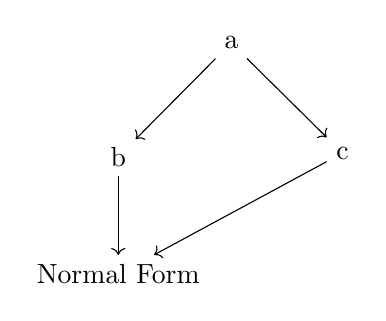
\begin{tikzpicture}
    \node (a) {a};
    \node (b) [below left=of a] {b};
    \node (c) [below right=of a] {c};
    \node (d) [below=of b] {Normal Form};
    \draw[->] (a) -- (b);
    \draw[->] (a) -- (c);
    \draw[->] (b) -- (d);
    \draw[->] (c) -- (d);
    \end{tikzpicture}
    
    \vspace{1cm}
    
    2. Confluent, Terminating, No Unique Normal Forms (True, True, False)
    \begin{tikzpicture}
    \node (a) {a};
    \node (b) [below left=of a] {b};
    \node (c) [below right=of a] {c};
    \node (d1) [below left=of b] {Normal Form 1};
    \node (d2) [below right=of c] {Normal Form 2};
    \draw[->] (a) -- (b);
    \draw[->] (a) -- (c);
    \draw[->] (b) -- (d1);
    \draw[->] (c) -- (d2);
    \end{tikzpicture}
    
    \vspace{1cm}
    
    3. Confluent, Not Terminating, Has Unique Normal Forms (True, False, True)
    \begin{tikzpicture}
    \node (a) {a};
    \node (b) [right=of a] {b};
    \node (c) [below right=of b] {c};
    \node (d) [below left=of c] {a};
    \draw[->] (a) -- (b);
    \draw[->] (b) -- (c);
    \draw[->] (c) -- (d);
    \draw[->] (d) -- (a);
    \end{tikzpicture}
    
    \vspace{1cm}
    
    4. Confluent, Not Terminating, No Unique Normal Forms (True, False, False)
    \begin{tikzpicture}
    \node (a) {a};
    \node (b) [below left=of a] {b};
    \node (c) [below right=of a] {c};
    \draw[->] (a) -- (b);
    \draw[->] (b) -- (a);
    \draw[->] (a) -- (c);
    \draw[->] (c) -- (a);
    \end{tikzpicture}
    
    \vspace{1cm}
    
    5. Not Confluent, Terminating, Has Unique Normal Forms (False, True, True)
    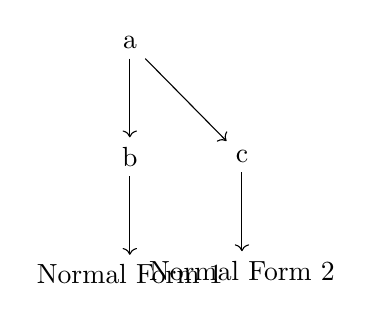
\begin{tikzpicture}
    \node (a) {a};
    \node (b) [below=of a] {b};
    \node (c) [right=of b] {c};
    \node (d) [below=of b] {Normal Form 1};
    \node (e) [below=of c] {Normal Form 2};
    \draw[->] (a) -- (b);
    \draw[->] (a) -- (c);
    \draw[->] (b) -- (d);
    \draw[->] (c) -- (e);
    \end{tikzpicture}
    
    \vspace{1cm}
    
    6. Not Confluent, Terminating, No Unique Normal Forms (False, True, False)
    \begin{tikzpicture}
    \node (a) {a};
    \node (b) [below left=of a] {b};
    \node (c) [below right=of a] {c};
    \node (d1) [below left=of b] {Normal Form 1};
    \node (d2) [below right=of c] {Normal Form 2};
    \draw[->] (a) -- (b);
    \draw[->] (a) -- (c);
    \draw[->] (b) -- (d1);
    \draw[->] (c) -- (d2);
    \end{tikzpicture}
    
    \vspace{1cm}
    
    7. Not Confluent, Not Terminating, Has Unique Normal Forms (False, False, True)
    \begin{tikzpicture}
    \node (a) {a};
    \node (b) [right=of a] {b};
    \node (c) [below right=of b] {c};
    \node (d) [below left=of c] {a};
    \draw[->] (a) -- (b);
    \draw[->] (b) -- (c);
    \draw[->] (c) -- (d);
    \draw[->] (d) -- (a);
    \end{tikzpicture}
    
    \vspace{1cm}
    
    8. Not Confluent, Not Terminating, No Unique Normal Forms (False, False, False)
    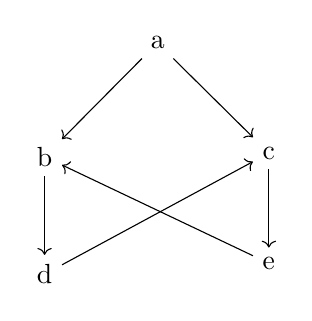
\begin{tikzpicture}
    \node (a) {a};
    \node (b) [below left=of a] {b};
    \node (c) [below right=of a] {c};
    \node (d) [below=of b] {d};
    \node (e) [below=of c] {e};
    \draw[->] (a) -- (b);
    \draw[->] (a) -- (c);
    \draw[->] (b) -- (d);
    \draw[->] (c) -- (e);
    \draw[->] (d) -- (c);
    \draw[->] (e) -- (b);
    \end{tikzpicture}

This weeks discord question is:

\begin{quote}
\small
 "In what ways might ARSs contribute to advancements in artificial intelligence, particularly in areas like automated reasoning or machine learning?"
\end{quote}
    
\section*{Conclusion}
In week one, we reviewed our discrete math knowledge and began coding proofs. Week two we saw the relationship between mathematical proofs and Lean code proofs, and then we began to solve problems recursively. In week three, I took a dive into quantum computing languages in my literature review while also working on coding a calculator using a recursive approach to solve parentheses. In week four, we explored parsing and context-free grammars, learning how to translate concrete syntax into abstract syntax, which is crucial for understanding how programming languages are processed. Week 5 used Lean as a way of proving logic puzzles. Week 6 built upon our logical foundations by focusing on implication in Lean Logic, proving logical statements. For week 7 we began to use lamda calculus to begin creating functions that could perform addition and multiplication. For weeks 8 and 9 we tackled a broken lambda calculus interpreter by identifying it's capture avoiding issues via the debugger. Week 10 we began to looking at ARS and breaking down how we reduce equations in a finite way. Week 11 we continued to look at ARS's and how to draw and describe them in order to understand how they work. 

\end{document}